\lhead{\emph{Related Work}}
\chapter{Related Work}

\section{\btree Indexes}

The \btree is a popular range index that has been adopted by SQL databases such as MYSQL and PostgreSQL \cite{kieseberg2019analysis}. Its structure is made up of internal and leaf nodes, with the internal nodes containing only indexes, and the leaf nodes containing all of the indexes \cite{comer1979ubiquitous}. Leaf nodes are linked together in a sequence set from left to right, which makes it possible to traverse the nodes in a specific order to retrieve data quickly and efficiently \cite{comer1979ubiquitous}.

One of the key advantages of the \btree is its ability to maintain height balance even when new data is inserted. This means that the depth of the left subtree is equal to that of the right subtree, ensuring that the search operation is efficient and the overall performance of the index is optimized \cite{comer1979ubiquitous}.

In addition to its height-balancing capabilities, the \btree is a dynamic data structure that can handle both read and write workloads. This makes it suitable for use in a variety of scenarios, including in-memory and on-disk storage \cite{comer1979ubiquitous}. Its versatility and reliability have made it a popular choice for developers and database administrators alike.

To search within a \btree, the operation involves traversing to the leaf node and then performing a binary search within the node \cite{comer1979ubiquitous}. This process allows for fast and efficient data retrieval, which is essential for applications that require real-time data processing.

Researchers have developed various methods to optimize the performance of \btree indexing, including taking advantage of hardware features such as CPU cache \cite{CSSCSBTree}, multi-core processors \cite{srinivasan1991performance}, and SIMD \cite{FAST}. These optimizations can significantly enhance the performance of the \btree in specific use cases.

Despite its general-purpose nature, the \btree can still be further optimized by taking into account existing data. Researchers have proposed machine learning-based techniques, such as learned indexes, that can leverage the statistical properties of the data to improve the performance of the \btree in edge cases \cite{CasedLearnedIndex}. By using these techniques, developers and database administrators can improve the performance of the \btree and optimize its use in specific applications.

\section{Tree-based Learned Index}
\begin{figure}
    \centering
    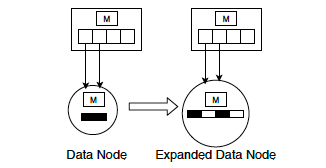
\includegraphics[width=100mm,scale=1]{Figures/alexNodeExpand.png}
    \caption{
     \acrlong{alex} node's expansion machanism.
    }
    \label{fig:alexNodeExpand}
\end{figure}
\subsection{Original Paper on Learned Index}
The \learnindex, a type of learned index structure, was first introduced in the paper titled "The Case for Learned Index Structures" by Tim Kraska \cite{CasedLearnedIndex}. Kraska's proposed method uses machine learning models to structure indexes and demonstrated its feasibility by creating a neural network using Python and TensorFlow. However, the study found that the neural network took $80,000ns$ to execute the model, while a standard B-tree only required $300ns$ for traversal and $900ns$ for the binary search. This discrepancy in execution time highlights the need for further optimization of the \learnindex structure.

Kraska identified three main factors that impact the query performance of the \learnindex. The first is the TensorFlow invocation overhead, which can be reduced through more efficient TensorFlow implementation. The second factor is the challenge of fitting cumulative distribution functions \acrfull{cdf} in neural networks as the \textsf{zoom-out} version may look smooth, but if looked closely, there may be more irregularities in the \acrshort{cdf}. Lastly, the third factor is the high cost of executing complex neural networks, which can be mitigated by using the right techniques.

To address the issue of overhead, Kraska introduced the Learning Index Framework (LIF), which is implemented in C++. LIF allows for the extraction of the neural network's weights and hyperparameters to avoid the framework overhead, thereby reducing the execution time. Additionally, to address the accuracy problem on non-smooth CDFs, Kraska introduced the \acrfull{rmi}. The \acrshort{rmi} is a hierarchical structure of models, where each model takes the key as input and predicts the next model to pick until the final stage, where it predicts the key's position. By using a hierarchical structure of models, \acrshort{rmi} can effectively reduce the number of parameters needed to achieve high accuracy.

Overall, Kraska's study and subsequent research into the \learnindex have demonstrated the potential for machine learning models to improve the performance of index structures. The use of LIF and \acrshort{rmi} has shown promising results in reducing overhead and improving accuracy, respectively. Further research in this area could lead to the development of even more efficient and accurate learned index structures, paving the way for exciting new developments in the field of database management.

\subsection{Static Learned Index}
\acrshort{rmi} is a static \learnindex. It forms a hierachy of models such that the underlying models more accurate representation of the \acrshort{cdf}. Experiments on \acrshort{rmi} shows that it outperforms the B-trees in the index size and the query speed. 

However, one limitation of \acrshort{rmi}, however, is that it only supports read operations. In modern systems, write operations are equally important, and optimizing the performance of both read and write operations is critical for achieving high database performance \cite{lourencco2015no}. Therefore, while the \acrshort{rmi} may offer benefits for read-optimized workloads, it may not be suitable for all applications.

Handling the updates in \acrshort{rmi} is challenging due to the data structure used and the operation is computationally expensive therefore degrading the performnance of the system. The \acrshort{rmi} can perform updates on keys but it has to shift the keys to the right to make space for the new key and also if the position of the keys are slightly modified, it will degrades the model's performance \cite{handlingupdates}. Most of \learnindex require a search within the error bound $\alpha$ to get the exact key position. For example, if \textsf{p} is the position predicted by the machine learning model, then the actual position of the key is within $[p-\alpha,p+\alpha]$. Hence using a binary search with the bounded error, $\alpha$ is guaranteed to get the actual position. Furthermore, re-training is required if there are too many shifts in the element's position or \acrshort{cdf} changes, which is slow when there is a large amount of data in the data structure \cite{ALEX}. 

Hybrid Learned Index (HLI) is another notable static learned index that offers significant performance benefits over traditional indexing structures. HLI is called hybrid because it combines two modules: the Piecewise Linear Approximation Model (PLA) with an error bound and the Rank-Model Index (RMI) without an error bound. The RMI is used to index the PLA-model, with the inner node structure being similar to RMI and ALEX. The leaf node in HLI is the PLA-model with an error bound. The main idea behind HLI is to use RMI to predict the segment that the keys belong to, then traverse until reaching the leaf node, which uses the PLA-model to predict the position.

One significant advantage of HLI is that it outperforms traditional indexing structures. In particular, it achieves up to $4.4\times$ the lookup performance of a B+tree. This performance boost is due to the use of a linear regression model as routing and the prediction only containing multiplication, which is bounded to $O(1)$. HLI also outperforms other learned indexes, such as RMI and PGM index, by about $50\%$.

However, there are some limitations to HLI. One significant drawback is that it does not support update operations such as insertion and deletion. This is because the PLA-model with error bound used in HLI is a static structure that cannot be updated. As a result, HLI is only suitable for scenarios where the data is static and not subject to frequent updates.

In summary, HLI is a static learned index that combines the RMI and PLA-model to achieve significant performance benefits over traditional indexing structures. The use of a linear regression model as routing and the prediction only containing multiplication, which is bounded to $O(1)$, makes HLI an efficient indexing structure. However, the lack of support for update operations limits the applicability of HLI to scenarios where the data is static and not subject to frequent updates.


\subsection{Hybrid Indexes}

In addition to the static learned index, Kraska also introduced the concept of hybrid indexes in his paper \cite{CasedLearnedIndex}. Hybrid indexes are a combination of the learned index and traditional index structures. By using the B-tree as the main index and incorporating the learned index, hybrid indexes aim to leverage the strengths of both methods. This combination can significantly improve the overall operation performance, especially for queries.

The learned index is used to predict the next child node such that it can jump to the next node directly, which improves the traversal process. However, if the distribution of the keys is difficult to learn, then the hybrid index falls back to using the traditional B-tree index. This hybrid approach provides a balance between the accuracy and performance of the index structure.

Moreover, hybrid indexes can benefit from the fact that the learned index can capture the patterns and dependencies among the keys, while the traditional index is efficient in handling updates. This combination provides a robust and flexible approach that can be adapted to different data distributions and scenarios.

The most notable hybrid indexes is called \acrshort{ftingtree} \cite{fittingtree}. The FIT-tree uses B+tree as its index structure. What makes it a learned index is that its leaf nodes contain the linear function to predict the position of the keys. When building the index, \acrshort{ftingtree} divides the keys into several segments, which then it will generate the linear function for each of the segment, which is stored in a B+tree. The key difference between \acrshort{ftingtree} and B+tree is that \acrshort{ftingtree} leaf nodes contain a predictor function while B+tree contains a key. When performing a query, B+tree will have to traverse down until the leaf node finds the particular key. On the other hand, \acrshort{ftingtree}'s leaf node does not contain keys, as it only contains the linear predictor function that represents each segment of the keys. To query in \acrshort{ftingtree}, first, it has to traverse down until the leaf node that represents a particular segment that the key located in. Secondly, it will have to perform a search for the key in the segment within the error bound $pred\_pos \pm err$. The error bound is defined difference between the predicted position and true position of a particular \cite{fittingtree}. 

In \acrshort{ftingtree}, keys are segmented which makes the process of segmenting very important. The algorithm \acrshort{ftingtree} uses is called "\textsf{ShrinkingCone}". It first forms a cone by defining an origin point, high slope ($sl_{high}$) and low slope ($sl_{low}$). The high slope and low slope represent the upper and lower bound of the segment. First the algorithm define $sl_{high} = \infty$ and $sl_{low} = 0$. Then if the key is inside the cone, then the high slope and low slope will be updated by using the key and key's position $\pm$ the \textsf{error}. In addition, the \textsf{ShinkingCone} is a non-optimal algorithm as it does not guarantee that it can produce the most optimal segment. However, there is still an upper bound on the maximum number of segments that the algorithm can produce $min(\frac{|keys|}{2}, \frac{|D|}{error+1})$ and $|D|$ is the number of datasets. This ensures that the amount \acrshort{ftingtree} will not produce more segments than the B+tree that uses a fixed size pages\cite{fittingtree}. 

From the experiment result \cite{fittingtree}, the \acrshort{ftingtree} shows an improvement over index with fixed-size paging in query performance while also memory efficient when compared to full and fixed-size paging index. Eventhough \acrshort{ftingtree} outperforms traditional indexes in lookup and space efficient, there is still some disadvantages of the \acrshort{ftingtree}. Firstly, the performance compared to the other learned index like previously mentioned \acrshort{rmi}. \acrshort{ftingtree} performance gained over B-tree is about $1.5\times$ while \acrshort{rmi} achieve almost $2\times$ the performance of query when compared to B-tree. Secondly, the insertion performance on \acrshort{ftingtree} does not outperform the full B-tree index in the insertion experiment \cite{fittingtree} as \acrshort{ftingtree} requires to perform splitting pages periodically and also performs a segmentation algorithm. 

Apart from \acrshort{ftingtree}, the \textsf{Interpolation-Friendly B-tree} (IFB-tree) is also another hybrid indexes \cite{ifb-tree}. Similar to \acrshort{ftingtree} the IFB-tree also uses B-tree with the node interpolation. The main idea is that node  interpolation is used to estimate the range that the keys located in. For example, if the look up key is $s$, then the interpolated index of $s$ is $\lfloor \frac{s-v_i}{v_{i+1} - v_i} \cdot n \rfloor$ where $v_i$ is the keys before $s$, $v_{i+1}$ is the key after $s$, and $n$ is the node size.

The main advantage of IFB-tree is that it does not consume any extra memory when compared to \acrshort{ftingtree}. \acrshort{ftingtree} requires storing parameters like slope and intercept for the linear regression function. The IFB-tree structure is B-tree which makes it light memory usage when compared to other hybrid indexes. 

However, the main drawback of the IFB-tree is similar to the \acrshort{ftingtree} that its query performs does outperforms a traditional B-tree but does not outperforms \learnindex like \acrshort{rmi}. Based on the result shown by Hadian \cite{ifb-tree}, the result is about up to $1.5\times$ the query performance of traditional B-tree, which is similar while the \acrshort{rmi} is almost $2-3\times$ faster on lookup performance compared to the traditional B-tree. However, if the result is compared to \acrshort{ftingtree}, there is barely any difference in term of lookup performance. The only benefit is that consumes lesser memory than the \acrshort{ftingtree}. 
 
\subsection{Dynamic Learned Index}
The \acrfull{alex} is a dynamic learned index structure proposed by Ding \cite{ALEX} that is designed to support both read and write operations such as insertion and deletion. In terms of structure, \acrshort{alex} is similar to the \acrshort{rmi} as it also has a hierarchy of models. The internal nodes only contain the linear regression model that points to the next child model to predict the partition of the keys. Meanwhile, the leaf nodes contain the keys and records in an array format. However, \acrshort{alex} uses a special data structure called the \textsf{Gapped Array} to store its keys and records in the leaf node.

The \textsf{Gapped Array} is a modified version of an array that leaves gaps between the keys instead of placing the empty spaces at the end of the array. This data structure enables \acrshort{alex} to use model-based insertion, where a model is used to predict the location of the new key, and insert it accordingly.

In addition to model-based insertion, \acrshort{alex} also employs node expansion and retraining to maintain its accuracy. To expand a node, the node must be $80\%$ full before performing the expansion. This criterion is checked when a new key is inserted. Furthermore, \acrshort{alex} performs shifting when a key already exists in the predicted position. It can shift to the right or left, depending on the closest gap.

However, if the distribution of new keys does not follow the existing distribution, the linear regression model becomes inaccurate, leading to a more densely packed region. This can deteriorate the shifting performance, which can take $O(n)$ in the worst case. To solve this issue, \acrshort{alex} requires expanding the data node or retraining the model.

One of the advantages of \acrshort{alex} is its ability to support update operations, which is crucial in real-world systems. This advantage addresses the shortcomings of static learned indexes by using the \textsf{Gapped Array} and model-based insertion.

Furthermore, the use of gaps in the \textsf{Gapped Array} ensures that the average cost of insertion and shifting elements is bounded to $O(\log m)$ instead of $O(m)$ if \acrshort{alex} has to shift keys to the closest gap.

Regarding the query operation, lookup in \acrshort{alex} consists of two stages. First, it traverses down until it reaches the leaf node, which costs $O(\log_m P)$. Secondly, it performs an exponential search as the keys may have shifted around, which costs $O(\log m)$. Since keys can be in any position within the error bound, an exponential search is required. Therefore, the total cost of a query becomes $O(\log_m P + \log m)$.

Overall, \acrshort{alex} is a dynamic learned index that supports both read and write operations with the use of the \textsf{Gapped Array} and model-based insertion. It also employs node expansion and retraining to maintain its accuracy, and its lookup operation has a worst-case time complexity of $O(\log_m P + \log m)$.

Aside from the \acrshort{alex} learned index, the Piecewise Geometric Model index (PGM index) is another dynamic index that aims to support read and write operations \cite{PGM}. The PGM index uses the Piecewise Linear Approximation Model, which segments the keys into multiple linear segments instead of using a machine learning model. This approach is different from \acrshort{ftingtree}, which stores keys in many nodes. However, the PGM index's structure is similar to \acrshort{alex}, with the main difference being in its model.

One of the advantages of PGM index is that it outperforms \acrshort{ftingtree} in terms of operational performance and memory consumption by up to $75\%$. It also dominates \acrshort{rmi} in terms of lookup and space consumption, and it even outperforms the B+tree in terms of space consumption. Moreover, the PGM index has a guaranteed worst-case bound, which is a significant advantage over the static learned index \acrshort{rmi}, as the latter lacks a guaranteed bound. The worst-case time complexity is $O(\log m_{opt} + \log \epsilon)$, and the space complexity is $\Theta(m_{opt})$. Here, $m_{opt}$ refers to the number of $\epsilon$-approximate segments. This makes the PGM index a superior dynamic learned index, as it can adapt based on the keys distribution, which may vary during lookup.

In addition, since the lookup operation is performed frequently in real-world systems, the PGM index's ability to adapt to different distributions during lookup makes it a very notable dynamic learned index. Furthermore, the PGM index also provides a smooth trade-off between operation performance and space consumption, allowing it to scale better in large datasets. In conclusion, the PGM index is a promising dynamic learned index that offers various advantages over other traditional and learned indexes. Future research can explore the PGM index's potential for further optimization and use in various real-world applications. 

RadixSpline is a dynamic learned index introduced by Kipf that uses spline interpolation and a radix table to perform efficient lookup \cite{kipf2020radixspline}. The index consists of two main components: a set of spline points and a radix table. The set of spline points is used to perform spline interpolation for any lookup key, resulting in a predicted position in the array. The radix table is then used to locate the accurate spline point for the queried key.

One of the advantages of RadixSpline is that it only has two hyperparameters to maintain: the number of radix bits $r$ and the spline error $e$. The $r$ parameter determines the size of the radix table and can be adjusted to balance accuracy and memory usage. A larger value of $r$ will increase the size of the radix table exponentially $2^r$, but it will also increase its accuracy.

Another advantage of RadixSpline is that it performs on par with traditional indexes in terms of build time. It is also competitive in terms of lookup performance when compared to other learned indexes. The index is built from the bottom up, constructing the error-bound spline on the keys and then indexing the spline points in the radix table.

However, RadixSpline has a significant drawback in that the radix table size $r$ must be tuned. This can be a challenge as the amount of data grows and the data distribution changes. If the value of $r$ is not carefully chosen, lookup performance can suffer.

Like other learned indexes, RadixSpline provides a good tradeoff between space and time complexity. It requires less space than traditional indexes while achieving comparable lookup performance. The use of spline interpolation also allows it to accurately predict the location of a key in the array, even if the key is not in the set of keys used to construct the index.



\acrfull{lipp} introduced by Jiacheng Wu to support update operations. The primary aim of \acrshort{lipp} is to predict the exact position of a key and eliminate any extra local search required to perform when the model miss predicts the location of the key \cite{LIPP}. The structure of nodes in \acrshort{lipp} is different from other dynamic learned indexes such as the \acrfull{alex}. Unlike the \acrshort{alex}, which has internal nodes and leaf nodes, \acrshort{lipp} only contains the data node, which consists of a gap, a pointer to the child node or a key.

One similarity between \acrshort{lipp} and \acrshort{alex} is that they both use Gapped Arrays in the index structure to reserve gaps for new key insertion. However, during the insertion operation, the main difference is that \acrshort{alex} shifts keys to the closest gaps available, while \acrshort{lipp} creates a new node and replaces the location as a pointer to the new node. The new node will have a gapped array with just two elements. However, the creation of a new node could grow the tree height, making the lookup operation time complexity to be bounded by $O(h)$, where $h$ is the height of the tree.

To solve this problem, \acrshort{lipp} has to perform adjustments (branch pruning) method that helps to reduce the amount of tree height such that it is bounded by the $O(\log N)$. It compares the number of nodes from the previous adjustments, and if it is $2\times$ more nodes than the previous adjustments, then \acrshort{lipp} will trigger the adjustments. Even though the lookup is still bounded by the height of the tree, the adjustment causes the lookup to have a shorter traversal path.

One of the main advantages of the \acrshort{lipp} index is that it outperforms both PGM index and \acrshort{alex} in read and write workloads by $13\times$ and $2.9\times$, respectively. Furthermore, \acrshort{lipp} also outperforms traditional indexes in the read and write operation as well. For the read-only workload, \acrshort{lipp} still outperforms \acrshort{alex}, PGM index, and \acrshort{rmi}. In addition, \acrshort{lipp} eliminates the last mile search completely by using the model to predict the precise position of the queried key.

However, \acrshort{alex} performs better in terms of memory consumption, as it uses gaps to shift the elements, while \acrshort{lipp} consumes extra memory when there is a conflict, as it has to hold two conflicting keys in the leaf nodes. Nonetheless, the \acrshort{lipp} index's benefits make it a promising solution for applications that require both high read and write performance.

In summary, \acrshort{lipp} is a dynamically learned index that uses a unique node structure and adjustments method to provide high read and write performance while eliminating the last mile search completely. Its performance in read and write workloads surpasses that of traditional indexes and other dynamic learned indexes such as \acrshort{alex} and PGM index, making it a promising solution for modern data-driven applications.

Dynamically learned indexes are becoming increasingly popular among researchers. However, these indexes require the presence of empty space, known as gaps, to facilitate the insertion of new elements. This presents a significant challenge in optimizing the algorithms that learn where to place the gaps to improve the efficiency of search and range queries while preserving the sorted order of the data to ensure the correctness of the range query.

However, the success of these methods depends on how well they learn to place the gaps. Poorly placed gaps can negatively impact the search and range query performance, leading to decreased efficiency and degraded accuracy. Therefore, there is a need for machine learning models or algorithms that can effectively learn where to place the gaps to optimize these indexes.


\section{Learned Hash Index}
Hash-table is a fundamental data structure used in many computer science applications, including database management systems. Its primary purpose is to provide an efficient way of looking up data by using a hash function to map keys to positions in an array. However, when two or more keys are mapped to the same position, a conflict occurs, and the hash-table needs to handle it. This is usually done by using a linked list to store all conflicting elements. While Hash-tables are efficient in lookup time, with an average lookup cost of $O(1)$, the worst-case lookup time can be as high as $O(n)$, where $n$ is the number of elements in the linked list.

To reduce the number of conflicts, various techniques have been developed, such as secondary probing or using multiple hash functions, like Cuckoo Hashing. While these techniques reduce the number of conflicts, conflicts can still impact lookup performance and memory consumption.

Kraska introduced the Hash-Model Index, which takes advantage of the underlying data distribution \cite{CasedLearnedIndex}. This index uses a machine learning model to learn the cumulative distribution function (CDF) of the data, providing a better hash function that reduces the number of conflicts by up to $77.5\%$. Unlike tree-based learned indexes, Hash-Model Indexes do not need to maintain sorted order, making them more suitable for supporting updates. When new items are inserted, they are stored in the array or a linked list if there is a conflict.

Hash-Model Indexes provide significant benefits over traditional Hash-tables, improving both lookup performance and memory consumption. Additionally, they provide a scalable solution that can handle large datasets efficiently. However, Hash-Model Indexes require more resources and computational power than traditional Hash tables, making them less suitable for applications with limited resources or computational power. 

\section{Multi-Dimensional Learned Index}
\begin{figure}
    \centering
    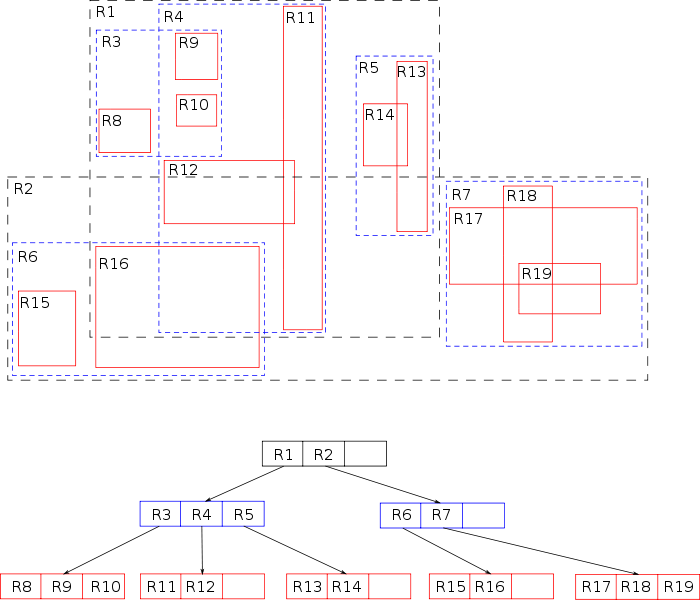
\includegraphics[width=100mm,scale=1]{Figures/R-tree.png}
    \caption{
        R-trees data structure and R-trees' bounding boxes 
    }
    \label{fig:R-tree}
\end{figure}
Scanning and filtering are two typical usages in a database engine \cite{FloodLMD}. To create an order, most database systems use a \btree index on a single attribute. However, when multiple attributes are filtered, using a \btree may lead to latency as the search has to follow pointers and narrow down the search space. To overcome this issue, multi-dimensional indexes with tree-based data structures such as R-trees \cite{r-tree} or k-d trees \cite{kdtree} can be used to improve the scanning performance of queries over multiple columns.

R-trees are a data structure that is commonly used for spatial data \cite{r-tree}. They support multi-dimensional indexing for objects such as geographical coordinates, rectangles, and polygons. R-trees group nearby objects and represent them using rectangular bounding boxes. This helps in reducing the search space during querying, which results in faster query execution times. The R-tree data structure is shown in Figure \ref{fig:R-tree}

In contrast, k-d trees divide the data into subregions using hyperplanes to group nearby points \cite{kdtree}. This approach is commonly used for nearest neighbor search, where the query searches for the data point closest to the given point.

Using multi-dimensional indexes with tree-based data structures provides an efficient solution for querying databases with multiple attributes. These data structures enable faster and more efficient searching by reducing the search space and optimizing the query execution time. As such, they are widely used in database engines for scanning and filtering operations.


Despite the advantages of using multi-dimensional indexes with tree-based data structures, such as R-trees \cite{r-tree} and k-d trees \cite{kdtree}, there are still some limitations that need to be addressed. One such limitation is the difficulty in tuning these indexes, which requires significant engineering efforts. Tuning the index for better performance in one scenario may not necessarily lead to better performance in another scenario \cite{FloodLMD}. Additionally, the indexes cannot adapt to specific workloads and data distributions, which may result in suboptimal performance.

In real-world scenarios, data distribution and query load can vary significantly, making it challenging to design an index that can adapt to changing conditions. Although traditional multi-dimensional indexes like R-trees and k-d trees are commonly used, they have their limitations. In particular, tuning these indexes for optimal performance can be a time-consuming and difficult task that requires significant engineering effort. Moreover, even when these indexes are properly tuned, their performance may not always be optimal, especially when dealing with skewed data distributions or heavy query workloads.

To address these issues, Flood index was developed as an in-memory learned multi-dimensional index that overcomes some of the limitations of traditional indexes \cite{FloodLMD}. Flood index is based on the concept of \acrfull{cdf}, which is used to learn the data distribution and project the multi-dimensional and skewed data into a uniform space. By doing so, the model can predict the data's location and provide fast access to it.

One of the main advantages of Flood index is that it outperforms traditional multi-dimensional indexes like R-trees and k-d trees by eliminating the need for search traversal times. Instead, Flood index relies on machine learning models to predict the location of the data. However, it should be noted that Flood index is designed to work only with read-only workloads. To support the insertion of new data, Flood index can leave gaps similar to \acrshort{alex} or \btree. 

Despite its usefulness, Flood suffers from two major drawbacks: it is not well-equipped to handle a query workload that is skewed \cite{Tsunami}, and it does not maintain uniformly sized grid cells. To address these issues, the Tsunami was developed as an optimized extension of the Flood index \cite{Tsunami}. However, the problem of efficient key insertion persists. One potential solution to this problem is to use gap reservation, which can aid in subsequent key insertions \cite{FloodLMD}.



\section{Learned Bloom Filters}
\begin{figure}
    \centering
    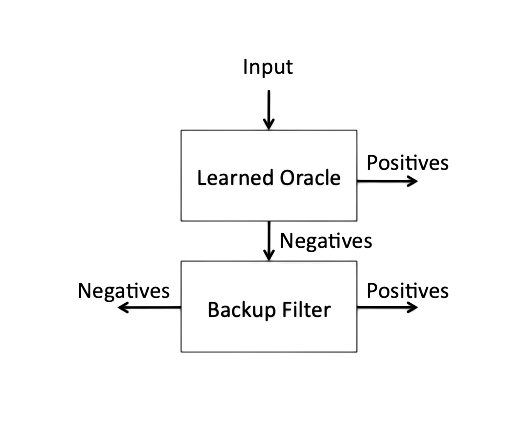
\includegraphics[width=80mm,scale=1]{Figures/learnedBloom.png}
    \caption{
        Learned oracle with backup Bloom filter (backup filter).
    }
    \label{fig:LearnedBloom}
\end{figure}
The Existence index, utilizing a Bloom filter, is one of the most widely used types of indexes in storage systems, databases, and other applications where the fast and efficient determination of set membership is essential. A Bloom filter is a probabilistic data structure that allows for checking if a key is present in a set with an extremely low false negative rate. It does this by utilizing a bit array of size $m$ and $k$ hash functions to map keys to $m$ array positions.

To add an element to the set, the key is inserted into the $k$ hash functions, which returns $k$ different positions in the $m$ array. The bits in these returned positions are then set to $1$, indicating the existence of the corresponding key in the set. During the insertion of a new key, the key is placed into the $k$ hash functions, and the resulting positions in the $m$ array bits are checked to determine if they are all $1$, indicating the presence of the key in the set.

One of the primary advantages of using a Bloom filter is its speed and efficiency in checking for set membership. For instance, Postgres, a popular open-source relational database management system, utilizes a Bloom filter index that allows for the fast exclusion of non-matching tuples \cite{postgresqlBloom}. Bloom filters are also space-efficient as they only require a fixed amount of memory for a given false positive rate.

However, Bloom filters do have a potential drawback, namely the possibility of false positives. A false positive occurs when the filter returns that a key is in the set when it is not. This happens when the hash functions of two different keys result in the same bit positions in the bit array, causing the filter to erroneously report that the key is present. The probability of a false positive is dependent on the size of the bit array $m$, the number of hash functions $k$, and the number of keys inserted into the Bloom filter.

Bloom filters have been found to be highly effective in many applications that require fast and efficient membership checking. However, there are some limitations to traditional Bloom filters, such as their potential for false positives, as discussed earlier. One potential solution to this problem is to augment Bloom filters with machine learning models, as proposed in the Learned Bloom filter \cite{LearnedBloom}.

The Learned Bloom filter is a probabilistic data structure that uses machine learning to make predictions about set membership. However, unlike traditional Bloom filters, the Learned Bloom filter does not provide a zero false negative rate. In other words, there is a chance that the machine learning model will not predict the correct value for a key. To overcome this limitation, the Learned Bloom filter requires a backup Bloom filter that can validate any false predictions made by the machine learning model (as shown in Figure \ref{fig:LearnedBloom}).

It is worth noting that the backup Bloom filter only needs to contain at most $FNR \times n$ elements, where $FNR$ is the false negative rate of the Learned Bloom filter and $n$ is the number of items in the set \cite{LearnedBloom}. This means that if the backup filter contains all the values similar to the traditional filter, it will take up more memory space as it needs to maintain both the backup filter and the Learned Bloom filter. By using this strategy, Bloom filters can potentially save memory space by storing only $n$ bits of elements.

In addition to the Learned Bloom filter, another approach to reducing the false positive rate of Bloom filters is the Sandwich Bloom filter. The Sandwich Bloom filter consists of two layers of Bloom filters, with the Learned Bloom filter sandwiched between them \cite{SandWichBloomFilter}.

The first layer of the Sandwich Bloom filter is the pre-filter, which is a traditional Bloom filter used to eliminate as many false positives as possible before the query reaches the Learned Bloom filter. The pre-filter reduces the workload of the Learned Bloom filter and helps to improve its accuracy. The pre-filter uses a set of independent hash functions to map keys to positions in the bit array, and each position is set to 1. When a key is queried, the pre-filter checks whether all of the corresponding positions in the bit array are set to 1. If any position is not set to 1, the query immediately returns false.

The second layer of the Sandwich Bloom filter is the backup filter, which is a traditional Bloom filter that is used to eliminate false negatives introduced by the Learned Bloom filter. As with the Learned Bloom filter, the backup filter only needs to store at most $FNR \times n$ elements, where $FNR$ is the false negative rate of the Learned Bloom filter and $n$ is the number of items in the set.

By sandwiching the Learned Bloom filter between the pre-filter and the backup filter\cite{SandWichBloomFilter}, the Sandwich Bloom filter can provide high accuracy while minimizing false positives and false negatives. However, like the Learned Bloom filter, the Sandwich Bloom filter is not perfect and may still produce errors. It is important to carefully evaluate the specific requirements of the application before choosing to use a Sandwich Bloom filter.

\section{Data Structure with Gaps}
\begin{figure}
    \centering
    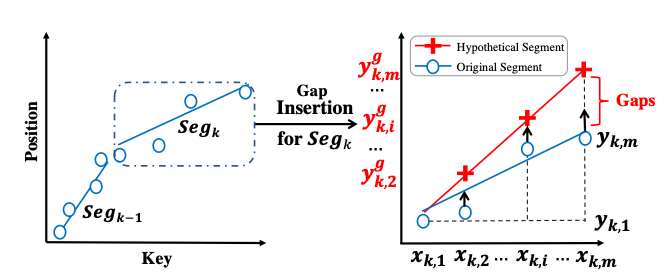
\includegraphics[width=120mm,scale=1]{Figures/gapsinsert.png}
    \caption{
        Gaps Insertion \cite{GapsInsertion}
    }
    \label{fig:gapsinsert}
\end{figure}

The concept of utilizing empty space, also known as gaps, for efficient insertion and deletion operations while maintaining the sorted order of keys is a common approach in various data structures, including the \learnindex\cite{ALEX,LIPP,PGM,fittingtree,FloodLMD,Tsunami, GapsInsertion}. The initial introduction of gaps in data structures can be traced back to \acrshort{alex}, where the \textsf{Gapped Array} technique was introduced. However, since then, several other data structures have utilized the concept of gaps, indicating its importance in designing efficient data structures.

For instance, the ubiquitous B+tree data structure, introduced by Comer in 1979, uses gaps at the end of its leaf nodes to allow for subsequent key insertion without significant overhead \cite{comer1979ubiquitous}. Another example of gap utilization is in the Packed Memory Array, a data structure designed for efficient searching and insertion of elements in compressed arrays, which also employs the use of gaps \cite{PackedMemoryArray}. Similarly, the Packed Memory Quadtree, a variant of the Packed Memory Array designed for two-dimensional spatial data, uses gaps to maintain a balanced tree structure and ensure efficient insertion and deletion operations \cite{packedquadtree}.

Another data structure, the \acrshort{ftingtree}, employs gaps at the end of its array to accommodate new key insertions and deletion operations while still guaranteeing a bounded error in query results \cite{fittingtree}. The \acrshort{ftingtree} shifts keys either left or right, depending on the closest gap, to maintain a balanced tree structure while still achieving optimal query performance.

In addition to reserving space for new data, gapping can also be used strategically to reduce conflicts and improve the efficiency of data structures. For instance, \acrshort{alex} places gaps in a way that reduces the number of conflicts between keys, which in turn minimizes the number of shifts required during insertion. This approach helps to reduce the worst-case shifting time to $O(m)$, where $m$ is the number of keys in the gapped array \cite{ALEX}.

Similarly, the LIPP tree \cite{LIPP} uses gaps to create new child nodes, which can improve the efficiency of the data structure. The PGM-index also uses gaps to reduce the size of its index and improve query times \cite{PGM}. The Tsunami index extends the Flood index by using gaps to maintain uniformly sized grid cells, which in turn improves the query performance \cite{Tsunami}.

Therefore, gapping is a widely used technique in various data structures to ensure efficient insertion and deletion operations while maintaining sorted keys.

\section{A Brief Summary}
The mutable \acrfull{tbli} have been shown to be effective in supporting insert operations while maintaining sorted keys by utilizing gaps. However, as we have observed from previous studies, conflicts arise when space is already occupied, leading to additional computation during insertion operations. To address this challenge, it is crucial to strategically place gaps in the array based on the available information, such as the distribution of existing data. In this project, we aim to minimize the number of conflicts in the \acrshort{lipp} \acrshort{tbli} by leveraging the information about the distribution of existing data, thereby optimizing the insertion overhead caused by conflicts. By strategically placing gaps, we aim to reduce the number of shifts and ensure that the model's error bound is still satisfied, leading to improved performance of TBLIs.

